\section*{Полнота Викиданных}

По данным категории \href{https://ru.wikipedia.org/wiki/%D0%9A%D0%B0%D1%82%D0%B5%D0%B3%D0%BE%D1%80%D0%B8%D1%8F:%D0%9A%D0%BE%D0%BC%D0%BF%D0%B0%D0%BD%D0%B8%D0%B8_%D0%BF%D0%BE_%D0%B0%D0%BB%D1%84%D0%B0%D0%B2%D0%B8%D1%82%D1%83}{Компании по алфавиту} Русской Википедии существует, как минимум, 10 272 коммерческие организации. Их количество изменяется с каждым днем (обычно, увеличивается) ввиду появления новых организаций, которые заносятся в данный список.

По данным категории \href{https://en.wikipedia.org/wiki/List_of_companies_of_Russia}{List of companies of Russia} Английской Википедии в Росиии существует как минимум 208 коммерческих организаций. В этой категории перечислен рейтинг крупнейших компаний России по объему реализации продукции. Можно сделать вывод, что даже крупные организации(Яндекс, Тинькофф) не вошли в данный список, не говоря уже про мелкие и средние.

Невозможно получить релевантные данные о количестве коммерческих организаций, так как их количество растёт с каждым днём, а данные о них не хранятся в открытом доступе. Взять, к примеру, Единый государственный реестр юридических лиц(ЕГРЮЛ), который предоставляет данные за плату \cite{egrul}.

"Количество коммерческих организаций, внесенных в госреестр как вновь созданных, в 2014 году составило 420,5 тыс."  свидетельствуют данные на сайте Федеральной налоговой службы России. З0 июня 2015 года вступили в силу приказы Минфина России о том, что данные об имеющихся организациях и информация по ним больше не распространяется в открытом доступе. Данные могут быть предоставлены только органам государственной власти, иным государственным органам, органам местного самоуправления и так далее. Поэтому получить достоверные данные о количестве имеющихся организаций не представляется возможным.

Оценим полноту информации о коммерческих организациях на Викиданных. Необходимо вспомнить цифру, полученную вначале, об общем количестве организаций на Викиданных (около 110 000). Найдем иллюстрации, соответствующие организациям с помощью запроса из листинга \ref{orgsimages}.

\begin{lstlisting}[language=SPARQL,label=orgsimages,caption=Организации с изображением]
#List of organizations with image

SELECT ?org ?orgLabel ?image
WHERE
{
  ?org wdt:P31 wd:Q4830453. #instance of orgs
  ?org wdt:P18 ?image #has image
  
  SERVICE wikibase:label { bd:serviceParam wikibase:language "en"}
}
\end{lstlisting}

\href{https://query.wikidata.org/#%23List%20of%20organisations%20%0A%0ASELECT%20%3Forg%20%3ForgLabel%20%3Fimage%0AWHERE%0A%7B%0A%20%20%3Forg%20wdt%3AP31%20wd%3AQ4830453.%20%23instance%20of%20orgs%0A%20%20%3Forg%20wdt%3AP18%20%3Fimage%0A%20%20%0A%0A%20%20SERVICE%20wikibase%3Alabel%20%7B%20bd%3AserviceParam%20wikibase%3Alanguage%20%22en%22%7D%0A%7D}{SPARQL-запрос}, 2913 записей.

Количество организаций с изображением равно 2 913, что составляет 3% от всех организаций. Это не так уж и много, что говорит о неполноте информации.

Оценим количество заполненных свойств у коммерческих организаций на Викиданных. Результат в табл. \ref{wdqueries}. Например inception(Дата создания) указано у 31 организаций, что составляет 31% от общего количества организаций.

\begin{table}[h]
\centering
\begin{tabular}{|l|l|}
\hline
\textbf{Имя свойства} & \textbf{Количество результатов} \\
\hline
inception (Дата создания) & 30995 \\	
\hline
founded by (Кем основана) & 5722 \\
\hline
subsidiary (Дочерние организации) & 3398 \\
\hline
image (Изображение) & 2913 \\
\hline
location (Географические координаты) & 577 \\
\hline
motto (Девиз) & 2 \\
\hline
\end{tabular}
\caption{Свойства объекта \enquote{Коммерческая организация} на Викиданных и их заполненность.}
\label{wdqueries}
\end{table}

Результаты данной таблицы (табл. \ref{wdqueries}) говорят о том, что количество необходимой информации об организациях очень мало, учитывая их общее количество на Викиданных. 

Исследуем полноту представления российских организаций в Викиданных (листинг \ref{rusorgs2}).

\begin{lstlisting}[language=SPARQL,label=rusorgs2,caption=Организации России]
#List of organizations 

SELECT ?org ?orgLabel
WHERE
{
  ?org wdt:P31 wd:Q4830453. #instance of organizations
  ?org wdt:P17 wd:Q159. #Russia country

  SERVICE wikibase:label { bd:serviceParam wikibase:language "en"}
}
\end{lstlisting}

\href{https://query.wikidata.org/#%23List%20of%20organisations%20%0A%0ASELECT%20%3Forg%20%3ForgLabel%20%3Flocation%0AWHERE%0A%7B%0A%20%20%3Forg%20wdt%3AP31%20wd%3AQ4830453.%20%23instance%20of%20orgs%0A%20%20%3Forg%20wdt%3AP17%20wd%3AQ159.%20%23Russia%20country%0A%0A%20%20SERVICE%20wikibase%3Alabel%20%7B%20bd%3AserviceParam%20wikibase%3Alanguage%20%22en%22%7D%0A%7D}{SPARQL-запрос}, 577 записей.

В Викиданных представлено 577 отечественных организаций Отобразим на карте те российские организации, у которых указан географические координаты (листинг \ref{rusorgsmap}).

\begin{lstlisting}[language=SPARQL,label=rusorgsmap,caption=Карта организаций России]
#Map of organizations 
#defaultView:Map

SELECT ?org ?orgLabel ?location
WHERE
{
  ?org wdt:P31 wd:Q4830453. #instance of orgs
  ?org wdt:P17 wd:Q159. #Russia country
  ?org wdt:P625 ?location #display location

  SERVICE wikibase:label { bd:serviceParam wikibase:language "en"}
}
\end{lstlisting}

\href{https://query.wikidata.org/#%23List%20of%20organisations%20%0A%23defaultView%3AMap%0A%0ASELECT%20%3Forg%20%3ForgLabel%20%3Flocation%0AWHERE%0A%7B%0A%20%20%3Forg%20wdt%3AP31%20wd%3AQ4830453.%20%23instance%20of%20orgs%0A%20%20%3Forg%20wdt%3AP17%20wd%3AQ159.%20%23Russia%20country%0A%20%20%3Forg%20wdt%3AP625%20%3Flocation%0A%0A%20%20SERVICE%20wikibase%3Alabel%20%7B%20bd%3AserviceParam%20wikibase%3Alanguage%20%22en%22%7D%0A%7D}{SPARQL-запрос}, 9 записей.

В результате оказалось очень мало записей с географическими координатами в России. Получить карту организаций не только России, но и всех организаций в мире можно с помощью следующего скрипта (листинг \ref{orgsmap}).

\begin{lstlisting}[language=SPARQL,label=orgsmap,caption=Карта организаций мира]
#List of organizations 
#defaultView:Map

SELECT ?org ?orgLabel ?location
WHERE
{
  ?org wdt:P31 wd:Q4830453. #instance of orgs
  ?org wdt:P625 ?location

  SERVICE wikibase:label { bd:serviceParam wikibase:language "en"}
}
\end{lstlisting}

\href{https://query.wikidata.org/#%23List%20of%20organisations%20%0A%23defaultView%3AMap%0A%0ASELECT%20%3Forg%20%3ForgLabel%20%3Flocation%0AWHERE%0A%7B%0A%20%20%3Forg%20wdt%3AP31%20wd%3AQ4830453.%20%23instance%20of%20orgs%0A%20%20%3Forg%20wdt%3AP625%20%3Flocation%0A%0A%20%20SERVICE%20wikibase%3Alabel%20%7B%20bd%3AserviceParam%20wikibase%3Alanguage%20%22en%22%7D%0A%7D}{SPARQL-запрос}, 511 записей.

Результат (рис. 3), опять-таки, очень скромный, всего лишь 511 организаций. Количество выведенных организаций с координатами даже меньше, чем общее количество всех организаций в России.

\begin{figure}[h]
	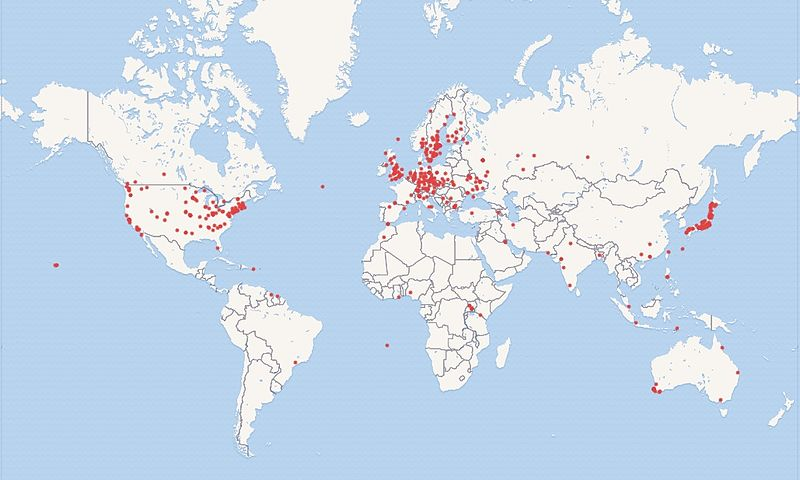
\includegraphics[scale=0.7]{World_organizations_map.jpg}
	\centering
	\caption{Карта организаций мира}
	\centering
\end{figure}

Проанализировав полученные данные, можно сделать вывод, что данные об организациях на Викиданных заполнены лишь частично. Не имеется достаточной информации, чтобы делать какие-то определенные выводы насчет организаций и их составляющих. Наличие авторитетных источников, неаффилированных и общедоступных крайне мало, а это главный козырь для создания статьи об организации в Википедии и Викиданных.. Но информация даже о таких крупнейших организациях (Apple, Microsoft, Intel) не полна и нуждается в доработке (например, у организации Intel не указан девиз).